\chapter{Resultados}
\label{section:Resultados}
Este capítulo apresenta os resultados das diversas etapas do fluxo proposto, bem como a análise dos mesmos. Alguns resultados preliminares foram utilizados para verificar se o trabalho está coerente com a base teórica anteriormente exposta. Outros auxiliaram na análise do fluxo de envelhecimento e na acuidade dos métodos de estimativa propostos.

Algumas considerações precisam ser feitas antes da análise dos dados. O ambiente de simulação criado para este trabalho reutiliza as ferramentas de EAD disponíveis para degradação, sendo sua integração realizada através de um conjunto de \textit{scripts}, que são responsáveis por automatizar:
\begin{enumerate}
	\item A criação das diversas netlists utilizadas no fluxo;
	\item Formatação dos arquivos utilizados como banco de dados bem como preenchimento dos mesmos;
	\item A passagem de parâmetros de entrada às ferramentas de EAD;
	\item A extração dos resultados de simulação;
	\item A atualização do banco de dados com as estimativas de MTTF.
\end{enumerate}

\section{Caracterização de células}
\label{section:caracterização}
Para investigar a relação entre as condições ambientais e a degradação de sistemas, é preciso averiguar primeiramente se é possível reproduzir resultados que estejam coerentes com a literatura. Isso significa que é necessário garantir que, ao se degradar um sistema, as alterações nas condições ambientais (\textit{p.ex.} temperatura) sejam refletidas no sistema conforme o esperado. É bem estabelecido que uma alteração na tensão de alimentação $V_{DD}$ deve influenciar não só a operação dos dispositivos mas também na contribuição dos efeitos de degradação expostos na seção \ref{subsection_Conf_CI}.

Com este propósito foram caracterizadas as seguintes células básicas: INV (inversor), AND2, OR2, NOR2 e NAND2. Elas foram degradadas separadamente e um modelo foi criado para cada uma através de uma regressão linear simples. Todas as células foram submetidas a BDPEs estáticos e populados exclusivamente para estas simulações. Por estático, significa que a célula foi submetida a uma mesma temperatura e tensão ao longo de toda a simulação ao invés de uma BDPE com diferentes $T_{conj,X}$ e $V_{conj,Y}$. Cada BDPE possui 200 perfis e o tempo de degradação para todas as células é de 1 ano.

Foram criados 5 BDPE's diferentes, um para cada célula. Entretanto, todos os perfis foram gerados usando a mesma premissa: os valores de temperatura seguem uma distribuição normal de média $\mu = 80$ e desvio-padrão $\sigma=10$. Os valores de tensão também seguem uma distribuição normal, porém de média $\mu = 1.1$ e desvio-padrão $\sigma=0.2$. Foi escolhida uma média de 80$^{\circ}$C com o intuito de garantir uma contribuição significativa da temperatura na degradação. Já a média da tensão de alimentação de $1.1V$ está de acordo com os parâmetros da tecnologia dos transistores utilizados na simulação.
 
Uma vez simulados e os modelos extraídos, 

\begin{figure}[H]
\center
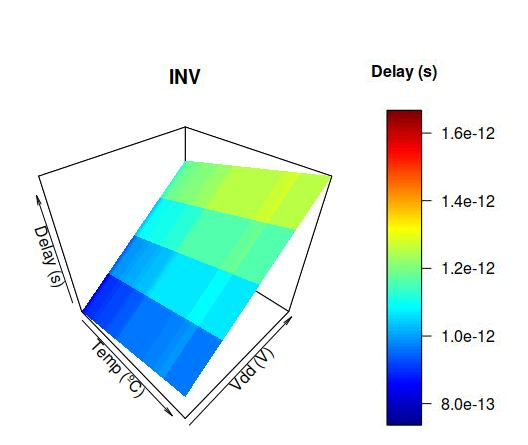
\includegraphics[width=0.9\textwidth]{images/delays_inv_caracterizacao_200Pontos_gauss80_10}
\caption{Caracterização de uma célula inversora após 1 ano de degradação.}
\label{delays_inv_caracterizacao_200Pontos_gauss80_10}	
\end{figure}
\begin{figure}[H]
\center
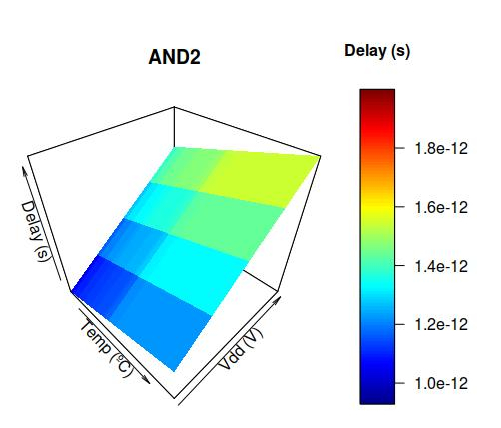
\includegraphics[width=0.9\textwidth]{images/delays_and2_caracterizacao_200Pontos_gauss80_10}
\caption{Caracterização de uma célula AND2}
\label{delays_and2_caracterizacao_200Pontos_gauss80_10}
\end{figure}
\begin{figure}[H]
\center
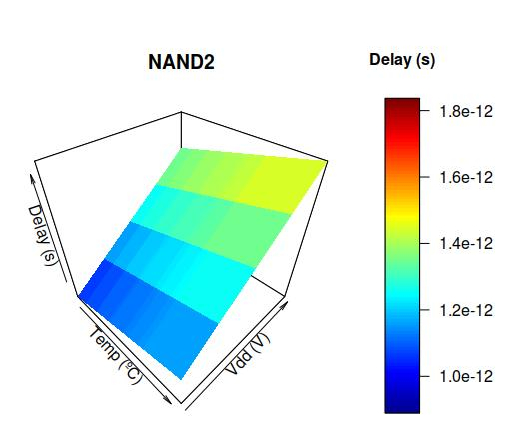
\includegraphics[width=0.9\textwidth]{images/delays_nand2_caracterizacao_200Pontos_gauss80_10}
\caption{Caracterização de uma célula NAND2}
\label{delays_nand2_caracterizacao_200Pontos_gauss80_10}
\end{figure}
\begin{figure}[H]
\center	
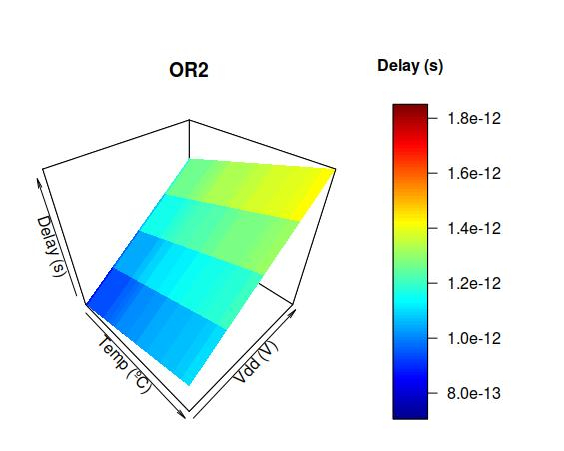
\includegraphics[width=0.9\textwidth]{images/delays_or2_caracterizacao_200Pontos_gauss80_10}
\caption{Caracterização de uma célula OR2}
\label{delays_or2_caracterizacao_200Pontos_gauss80_10}
\end{figure}
\begin{figure}[H]
\center
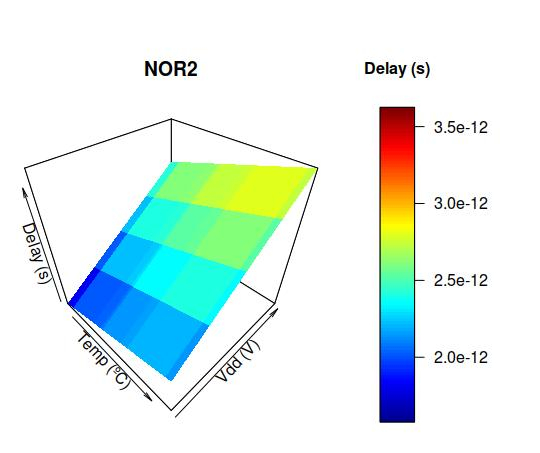
\includegraphics[width=0.9\textwidth]{images/delays_nor2_caracterizacao_200Pontos_gauss80_10}
\caption{Caracterização de uma célula OR2}
\label{figure:delays_nor2_caracterizacao_200Pontos_gauss80_10}]
\end{figure}

Foi realizada uma comparação entre delays absolutos e relativos para os diferentes métodos de estimativa foi aplicada a um inversor e a uma cadeia de inversores.


\section{Caracterização de circuitos de teste}
\label{section:caracterização_iscas}
São utilizados também uma cadeia de 100 (cem) inversores e quatro circuitos ISCAS-85: c499, c880, c1355, c5315. Esses circuitos ISCAS são implementações de blocos combinacionais pré-determinados cujo objetivo é propor um padrão para testes \cite{Hansen1999}. A função lógica e a quantidade de portas lógicas para cada um deles está descrita na tabela \ref{tb:ISCAS_85}.
\begin{table}[H]
\centering
\begin{tabular}{@{}lll@{}}
\toprule
Circuito & Função & Número de portas lógicas \\ \midrule
c499 & Single-Error-Correcting de 32-bit & 474 \\ \midrule
c880 & Ula de 8 bits & 393 \\ \midrule
c1355 & Single-Error-Correcting de 32-bit & 738 \\ \midrule
c5315 & Ula de 9 bits & 1781 \\ \bottomrule
\end{tabular}
\caption{Características dos circuitos combinacionais ISCAS-85 \cite{Hansen1999}.}
\label{tb:ISCAS_85}
\end{table}
Esses circuitos podem ser utilizados para os próximos passos em sua integridade ou apenas uma porção dos mesmos. Por integridade entende-se que os circuitos, inicialmente descritos através de uma linguagem de descrição de hardware (Hardware Description Language, HDL), serão sintetizados e o circuito obtido será utilizado na criação de uma netlsit Spectre. 

Por porção entende-se que somente uma parte do circuito será utilizada para criação da netlist Spectre. Esta parte deve ser capaz de, após as simulações de envelhecimento, representar o pior caso para o restante do circuito. Esta porção é representada por um mais caminhos críticos.

Uma vez criada, a netlist é padronizada com valores de temperatura $T$ e alimentação $V_{DD}$ de referência. Em seguida são criados N cópias da netlist desejada e seus valores de referência são substituídos pelos valores disponíveis de condições ambientais exemplificados pela tabela \ref{tb:BDPE_reduzida}.
\begin{figure}[H]
\center
\subfloat[MSE para ISCAS C499\label{figure:MSE_betw_3methods_worst_c499_Eucl_Corr_PLS}]{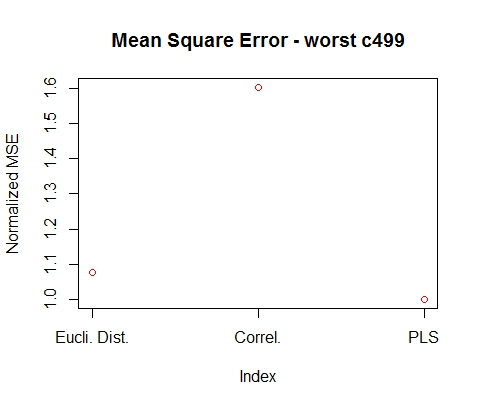
\includegraphics[width=0.3\textwidth]{images/MSE_betw_3methods_worst_c499_Eucl_Corr_PLS}
}
\hfill
\subfloat[MSE para ISCAS C880\label{figure:MSE_betw_3methods_worst_c880_Eucl_Corr_PLS}]{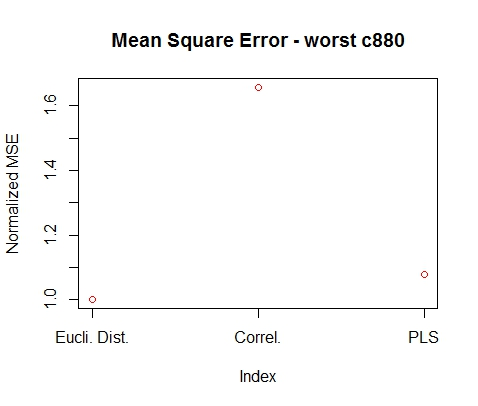
\includegraphics[width=0.3\textwidth]{images/MSE_betw_3methods_worst_c880_Eucl_Corr_PLS}
}
\hfill
\subfloat[MSE para ISCAS C1355\label{figure:MSE_betw_3methods_worst_c1355_Eucl_Corr_PLS}]{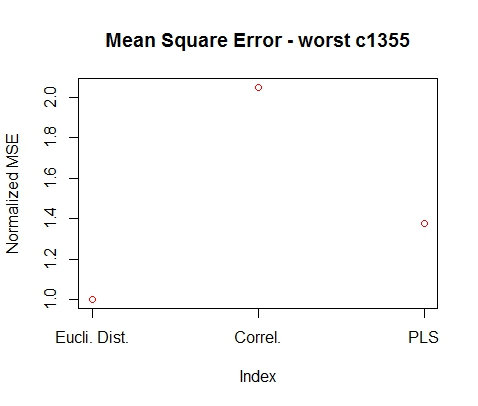
\includegraphics[width=0.3\textwidth]{images/MSE_betw_3methods_worst_c1355_Eucl_Corr_PLS}
}
\hfill
\subfloat[MSE para ISCAS C5315\label{figure:MSE_betw_3methods_worst_c5315_Eucl_Corr_PLS}]{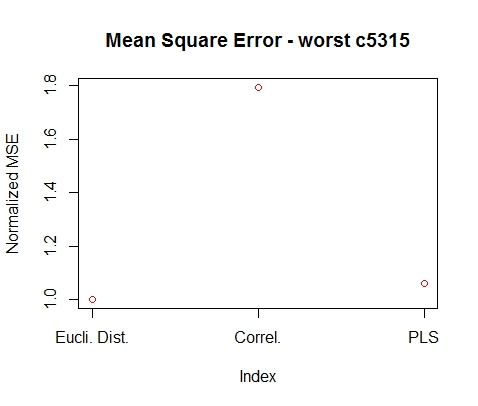
\includegraphics[width=0.3\textwidth]{images/MSE_betw_3methods_worst_c5315_Eucl_Corr_PLS}
}
\hfill
\subfloat[MTTF para ISCAS C499\label{figure:MTTF_ratio_percentage_worst_c499}]{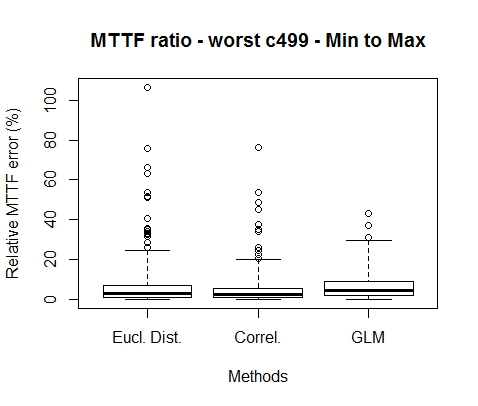
\includegraphics[width=0.3\textwidth]{images/MTTF_ratio_percentage_worst_c499}
}
\hfill
\subfloat[MTTF para ISCAS C880\label{figure:MTTF_ratio_percentage_worst_c880}]{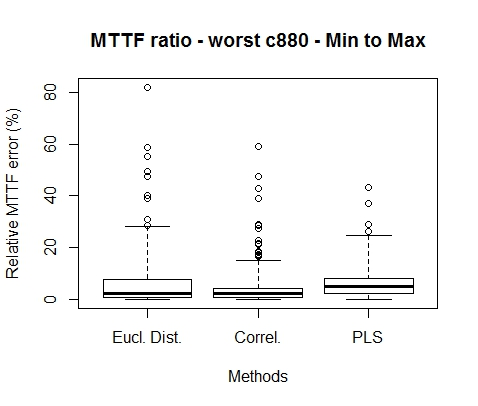
\includegraphics[width=0.3\textwidth]{images/MTTF_ratio_percentage_worst_c880}
}
\hfill
\subfloat[MTTF para ISCAS C1355\label{figure:MTTF_ratio_percentage_worst_c1355}]{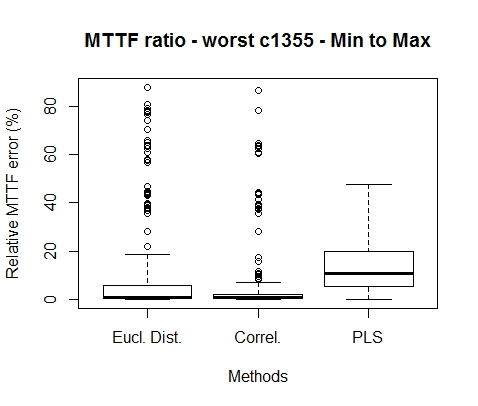
\includegraphics[width=0.3\textwidth]{images/MTTF_ratio_percentage_worst_c1355}
}
\hfill
\subfloat[MTTF para ISCAS C5315\label{figure:MTTF_ratio_percentage_worst_c5315}]{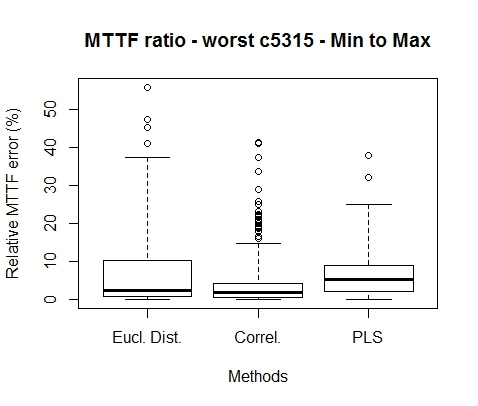
\includegraphics[width=0.3\textwidth]{images/MTTF_ratio_percentage_worst_c5315}
}
\caption{\textit{Mean Square Error} e \textit{Mean Time To Failure rate} entre métodos.\textcolor{red}{SEPARAR O GRÁFICO POR CIRCUITO?}}
\label{figure:mse}
\end{figure}

\section{Métricas e estatísticas}

\section{Discussão dos resultados}
Utiliza-se uma tabela de simulação para cada método, retira-se um dos pontos, treina-se o método utilizando os pontos restantes e testa-se a exatidão do modelo gerado estimando o atraso para o ponto que foi retirado anteriormente.
Com o erro quadrático de cada ponto, calcula-se o erro médio quadrático (\textit{Mean Square Error}, MSE) normalizado para os 3 métodos.

Isso já mostra que o método da correlação apresenta um erro maior do que o método da distância euclidiana. Já o GLM tem um taxa de erro 80\% menor do que a distância euclidiana.
